\documentclass[12 pt,a4 paper ]{scrreprt}
%---------------------------------------------------------- 
\usepackage[utf8]{inputenc}
\usepackage[naustrian]{babel}
\usepackage{lmodern}
\usepackage[T1]{fontenc}
\usepackage{graphicx}
\usepackage{amsmath}
\usepackage{float}
\usepackage{amsmath,amssymb,amstext}
\usepackage{pgfplots}
\usepackage{eurosym}
\usepackage{nicefrac}
\usepackage{units}
\usepackage{color}
%\usepackage[tight]{units}
%\usepackage[loose]{units}
\usepackage{pgfplots, pgfplotstable}
\usepackage[headsepline,plainheadsepline]{scrpage2}
\pagestyle{scrheadings}
\ihead[\rightmark]{\rightmark} \chead[]{}
%\ohead[\pagemark]{\pagemark} \cfoot[]{}
\usepackage{pgfplots, pgfplotstable}
\usepackage{tikz}
\usepackage{pgfplots}

\automark{chapter}
\renewcommand{\chaptermark}[1]{\markright{\ #1}}



\pgfplotsset{width=15cm,compat=1.6}
\usepackage{pgfplots}

 \usepackage[raiselinks]{hyperref}
\usepackage{amsfonts}  
\usepackage{babelbib} 
\usepackage{url} 
%\usepackage[fixlanguage]{babelbib}

\begin{document} 



\begin{figure}[h!]
\begin{center}
\begin{tikzpicture}
\begin{axis}[height=12cm, width=12cm,
			axis y line*=left, 
			no markers,
			xmajorgrids,ymajorgrids,
			xlabel=Zeit\,$\lbrack s \rbrack$,
			ylabel=Kraft\,/\,Zylinder\,$\lbrack kN\rbrack$,
			xmin=0,ymin=0,
			legend pos= north east,
			axis on top,			
			 ]
\addplot table[y=F,x=t]{Auswertung/1versuch/BT1.dat};
\legend{F};
\addlegendentry{BT1};
\end{axis}
\begin{axis}[height=12cm, width=12cm, 
			axis y line*=right,
			axis x line*=none,
			no markers,
			xmajorgrids,ymajorgrids,
			ylabel=Verschiebung\,u\,$\lbrack mm\rbrack$,
			xmin=0,ymin=0,
			legend pos=south east,axis on top						
			 ]
\addplot table[y=u1.1,x=t]{Auswertung/1versuch/BT1.dat};
\addplot table[y=u1.2,x=t]{Auswertung/1versuch/BT1.dat};
\addplot table[y=u2,x=t]{Auswertung/1versuch/BT1.dat};
\addplot table[y=u3,x=t]{Auswertung/1versuch/BT1.dat};
\legend{BT1\,u1.1,BT1\,u1.2,BT1\,u2,BT1\,u3};
\end{axis}
\end{tikzpicture}
\caption{Bauteilversuch 1: Kraft-Zeit}
\label{1 Versuch: Kraft-Durchbiegung}
\end{center}
\end{figure}


\begin{figure}[h!]
\begin{center}
\includegraphics[scale =0.9,trim= 1.5cm 10cm 1.5cm 10cm, clip=true]{Auswertung/1versuch/BT1.pdf}
\caption{Darstellung des BT\,1, mit Verbindungsmittel und Lasteinleiung}
\label{1versuch}
\end{center}
\end{figure}



\begin{figure}[h!]
\begin{minipage}[hbt]{7cm}
	\includegraphics[width=7cm]{Auswertung/1versuch/versuchsschema_scherversuch.png}
	\caption{Versuchsschema: Scherversuch nach []}
	\label{versuchsschema_scherversuch}
\end{minipage}
\hfill
\begin{minipage}[hbt]{7cm}
\includegraphics[scale=1.2, trim=4cm 12cm 11.5cm 9cm, clip=true]{Auswertung/schubversuch/Schubversuch_Skizze.pdf}
	\caption{Skizze des Schubversuchs}
	\label{abb:Skizze des Schubversuchs}
\end{minipage}
\end{figure}




\begin{figure}[h!]
\begin{center}
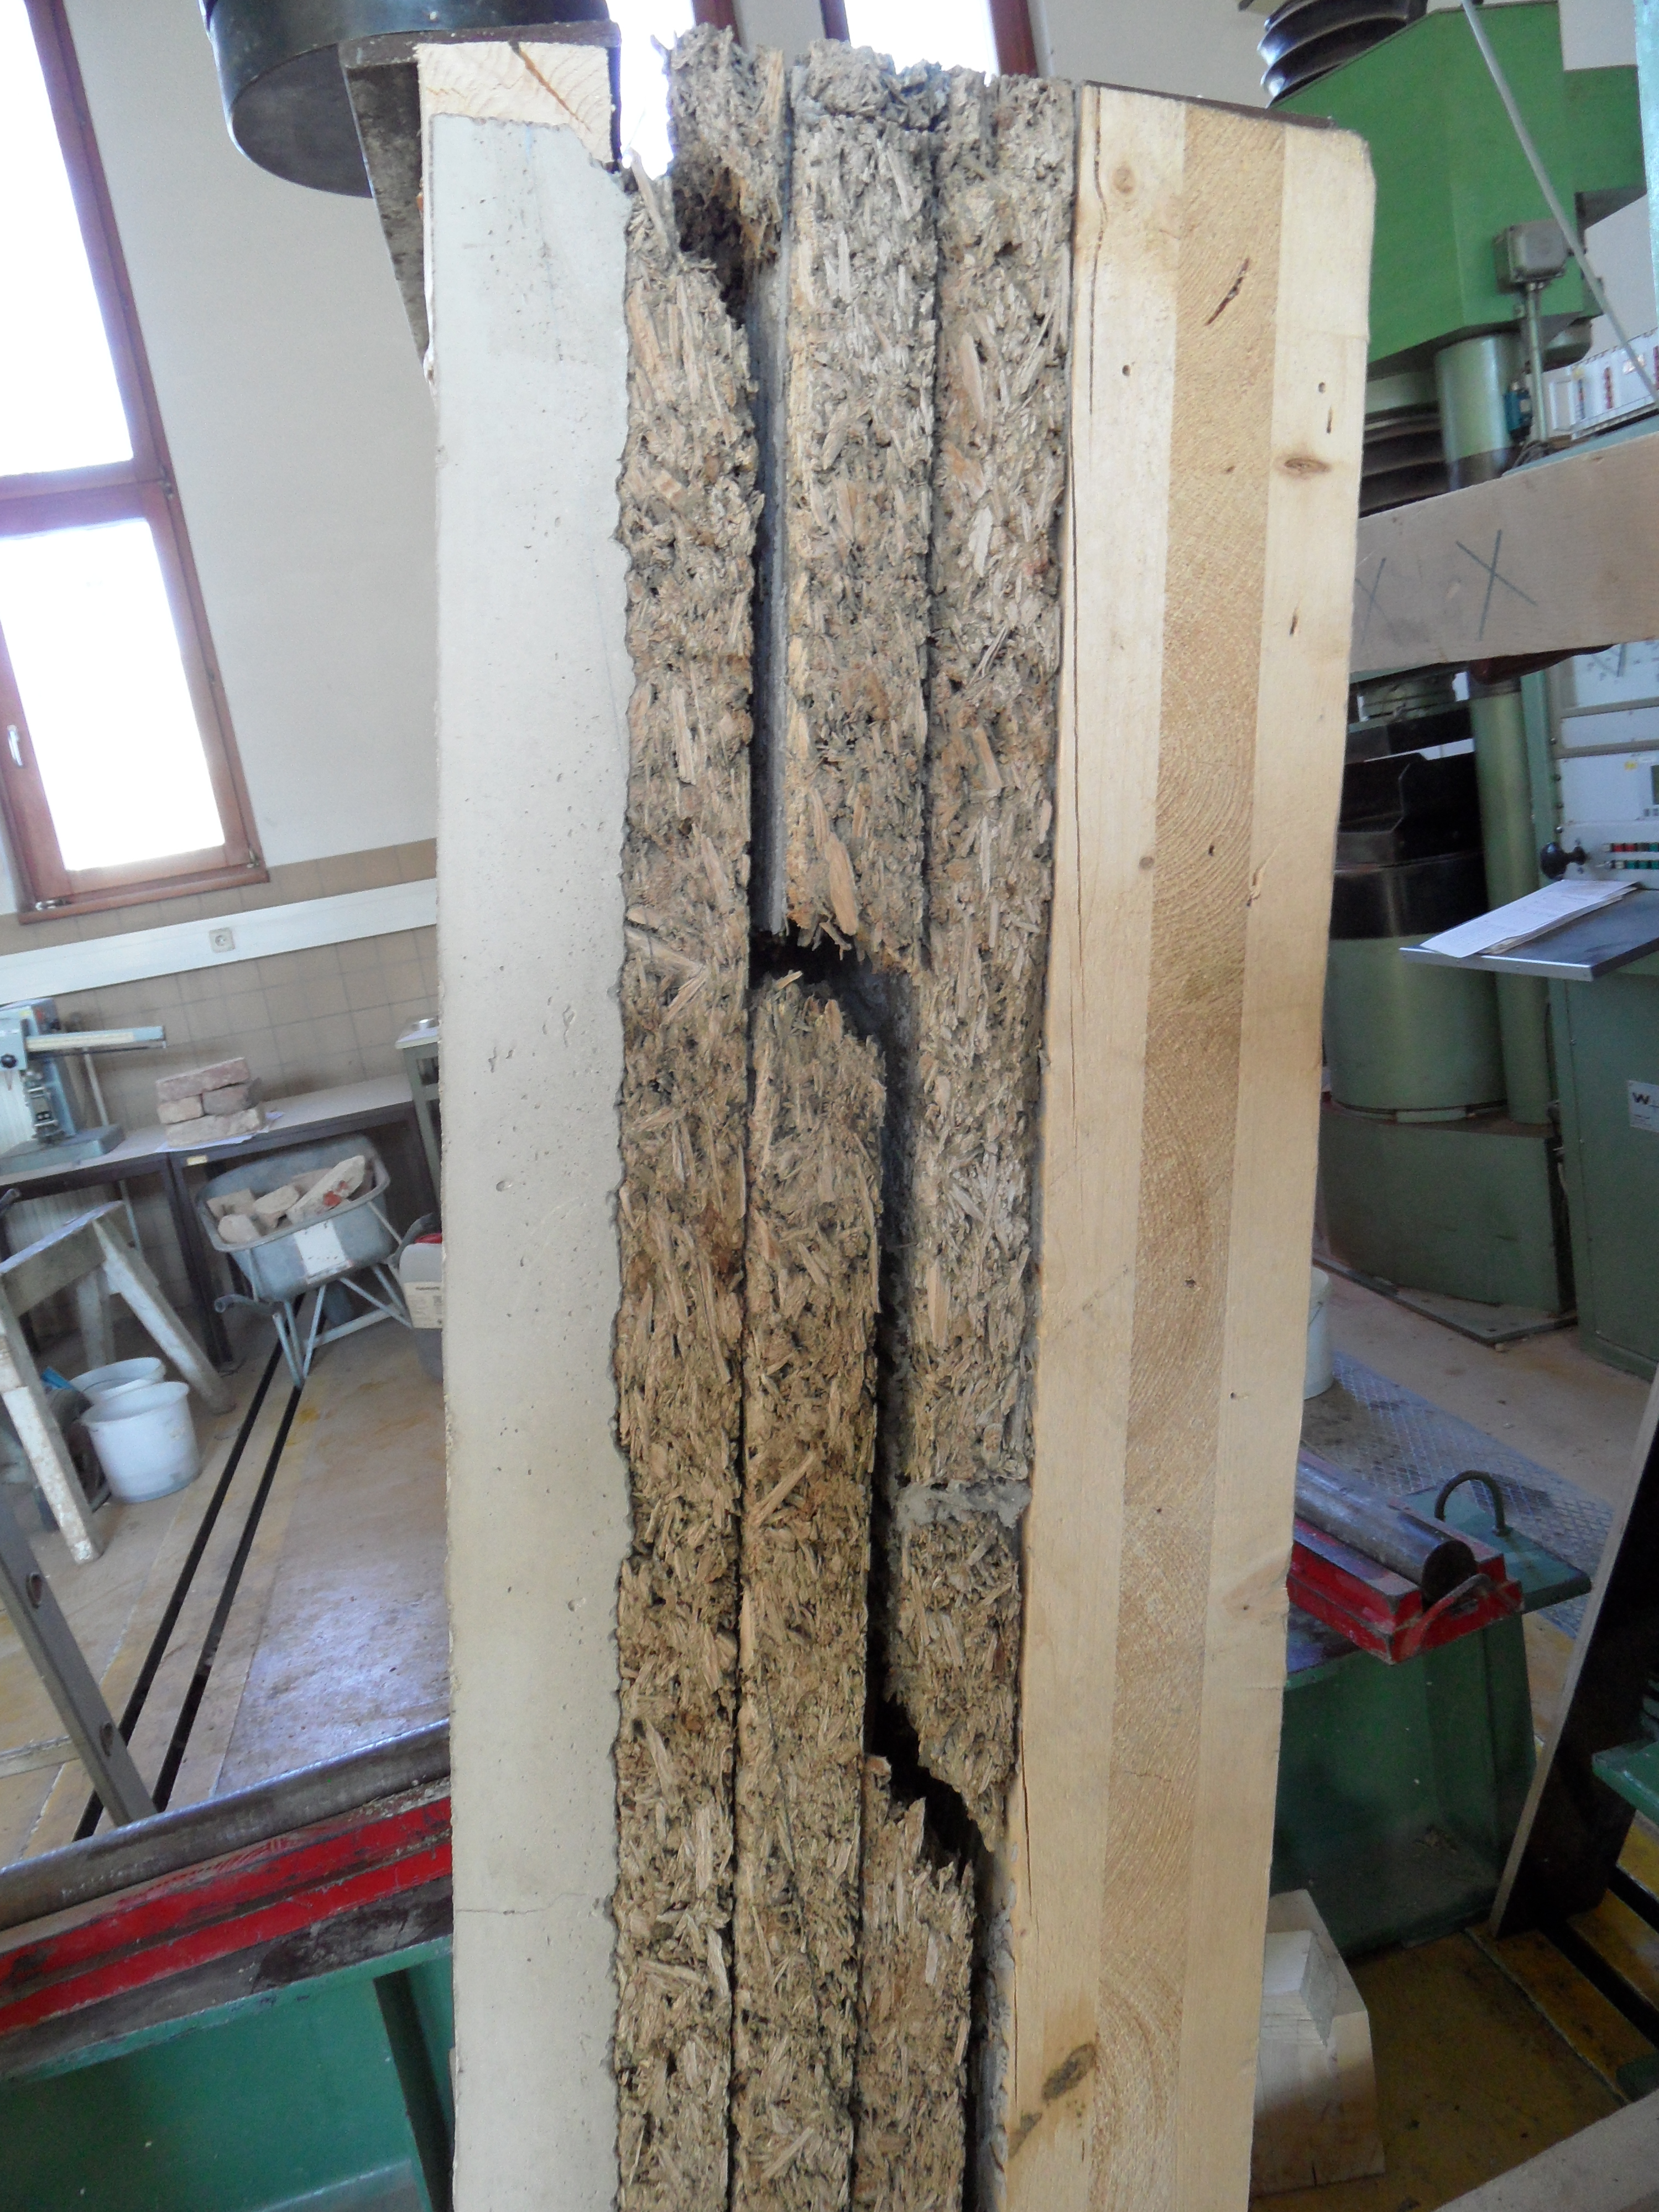
\includegraphics[scale =0.1]{Auswertung/schubversuch/SV_Bruchbild_seitlich.jpg}
\caption{Darstellung des BT\,1, mit Verbindungsmittel und Lasteinleiung}
\label{1versuch}
\end{center}
\end{figure}


\begin{table}[h]
\caption{Berechnung}
\begin{center}
\begin{tabular}{|c|c|c|c|c|}

\hline 
Versuch & $F_{max}$  & $F_{04}$ & $v_{04}$ & $k_{s,04}$  \\ 

&  [kN] & [kN] & [mm] & [N/mm]    \\ 
\hline\hline
SV1 & 359  & 144 & 1,17 & 123076    \\ 
\hline 
SV2 & 348  & 139 & 0,11 & 1263636   \\ 

\hline 
\end{tabular} 
\end{center}
\label{tab:Versuchsprogramm}
\end{table}

\begin{figure}
\begin{center}
\begin{tikzpicture}
\begin{axis}[legend pos= outer north east,
			height=12cm, width=12cm,
			ylabel= $\lbrack kN\rbrack $ /$\lbrack N/mm^2\rbrack $,
			ybar,
			enlargelimits=0.25,
			symbolic x coords={V1,V2,V3},
			xtick=data,
			nodes near coords
			]
\addplot coordinates {(V1,0.34) (V2,0.52) (V3,0.26)};

\addplot coordinates {(V1,0.56) (V2,0.46) (V3,0.64)};
\addplot [color=brown,fill=brown]coordinates {(V1,0.46) (V2,0.46) (V3,0.45)};
\addplot coordinates {(V1,) (V2,) (V3,)};
\addplot coordinates {(V1,0.17) (V2,0.26) (V3,0.13)};
\addplot[color=green,fill=green]coordinates {(V1,0.30) (V2,0.2) (V3,0.33)};
\addplot[color=blue,fill=blue] coordinates {(V1,0.23) (V2,0.23) (V3,0.23)};
\legend{Kraft\,1,Kraft\,2,Durchschnitt,Spannung\,1,Spannung\,2,Durchschnitt}
\end{axis}
\end{tikzpicture}
\caption{Bauteilversuch 3: Kraft-Durchbiegung}
\label{BT3_durchbiegung}
\end{center}
\end{figure}

\newpage 
babbabaablblablalbabla\cite{WRT}
\bibliographystyle{alphabetic} 
\bibliography{Verzeichnis.bib} 



Es scheint, dass der Anzahl der Schrauben in Bezug auf die Durchbiegung, nur einen geringen Einfluss hat. Der zweite Bauteil weist eine geringe Steigung auf, dass auf die Vorschädigung zurückzuführen ist. Durch die Verwendung des schlechteren Klebers und die Verminderung der Schraubenanzahl, kann der Abfall erklärt werden. Der vierte Bauteil hatte keine mechanischen Verbindungsmittel in Verwendung, daher waren auch schon vor dem Versuch bzw. beim einbringen in die Prüfmaschine, Schädigungen entstanden. 
Es ist festzustellen, dass das Sandwich ohne mechanische Verbindungsmittel, eine zu geringe Steifigkeit aufweist. Jedoch kann die Anzahl, auf ein Minimum gesetzt werden.


 Es kann die Annahme getroffen werden, dass die Anzahl der Schrauben keinen linearen Einfluss aufweisen.


Dies ist wiederum auf den Verzicht auf mechanische Verbindungsmittel zurück zu führen.






!!!!!!!!!!!!!!!!
\paragraph{BT2}
und erfuhr daher einen Lastzustand der nicht vorgesehen war. Durch das mittige Anhebung war ein Kragarm and den Enden  mit ca. \unit[2,0]{m} Länge entstanden. Womit sich die Zug und Druckzone umgekehrte. So entstanden die Risse im Beton. Das Abheben der oberen Veloxschichten ist auf den verwendeten Kleber und dessen ungenügende Klebeeigenschaften zurückzuführen (laut einer Expertenaussage (Hr. Rössler, Fa. Sika).
Es ist noch festzuhalten das beim 1 Bauteilversuch ident vorgegangen worden ist. Aufgrund der Verringerung der Schraubenanzahl und der Verwendung eines anderen Klebers, ist ein Bauteil entstanden, der eine geringe Steifigkeit hat. Dies ist der Grund für die Schädigung des Bauteils.





In den Abblindungen \ref{velos unten} und \ref{velox ober} sind die Oberflächen abgebildet, in der Mitte des Trägers. Es sind Teilflächen zu erkennen, welche noch die Riffen der Zahnspachtel aufweisen und Teilflächen auf der gegenüber liegenden Seite, keine Benetzung mit dem Kleber aufweisen. In diesen Bereich hat nie ein Verbund stattgefunden. Es liegt hier kein Versagen der Veloxschicht vor, ausschließlich von der Klebeschicht, da keine Spuren des Veloxmaterials auf der gegenüberliegenden Seite feststellbar waren. 



Vergleicht man die Kennlinien explizit nur in der Phase nach dem Plateau bzw. ab der Stelle, wo nur noch die Schrauben zur Lastableitung beitragen, ist die Kennlinie nahezu ident. Das heißt der Unterschied zwischen den Versuchskennlinien, kann auf die unterschiedliche Ausganglage (Vorschädigung) der Versuchskörper zurückführt werden. \newline
Das Tragverhalten des Holzleichtbetonschicht im Zusammenspiel mit den Schrauben muss noch mit weiteren Versuchen abgeklärt werden


	\subparagraph{Conclusio:}


Es ist ersichtlich, dass die beiden Versuche die fast gleiche Bruchlast aufweisen. Jedoch ist die Verschiebung beim zweiten Versuch um die Hälfte geringer. Der Verlauf der Kennlinie ist auch nicht ident, daher müssten verschiedene Mechanismen bei den  Versuchen unterschiedlich aufgetreten sein. 

Der Hauptgrund für die unterschiedliche Kennlinie ist die Vorbelastung durch den  4-Punkt-Biegeversuch. Auch wenn visuell keine Beeinträchtigung der Versuchskörper zu sehen war, hatte die Klebefuge bzw. die innere Festigkeit vom Velox, beim zweiten Versuch keinen Beitrag zur Lastabtragung. Somit musste die ganze Kraft über die Schrauben abgetragen werden.  Beim zweiten Versuch ist ein ausgeprägtes Plateau ersichtlich. Daher kann man davon ausgehen, dass vor dem Plateau die Schrauben und das Velox die Last abgetragen haben. Danach ist die Schraube alleine für die Lastabtragung verantwortlich. Die Steigung der Kennlinie bekräftigt die die oben beschriebene Vermutung, dass das System steifer ist als beim ersten Versuch. Beim zweiten Versuch ist die kein Plateau ersichtlich daher keine Beitrag vom Velox und somit eine geringe Steifigkeit des Systems.
Der Unterschied in den Verschiebung könnte durch die beschriebenen Steifigkeitsunterschiede abgeleitet werden. Die Schrauben werden beim 2 Versuch noch durch die intakte Verbundfuge 
unterstützt, daraus ergibt sich eine geringere Verschiebung, als in der ersten Phase des Versuchs.

\end{document}